\section{Infraestructura Cloud}
\label{sec:infraestructura}

Uno de los pilares de este trabajo es la demostración de la viabilidad económica del proyecto mediante el uso de infraestructura cloud optimizada y automatizada. La arquitectura de hardware seleccionada no solo responde a necesidades de rendimiento, sino que se integra en un flujo de despliegue continuo donde la intervención humana es mínima.

\subsection{Ecosistema AWS: Provisión de Recursos}
Para el despliegue del entorno de entrenamiento, se ha seleccionado Amazon Web Services (AWS) debido a su madurez en servicios de computación acelerada y su capacidad de ofrecer recursos de alto rendimiento bajo demanda.

\subsubsection{Repositorio de Imágenes: Amazon ECR}
Amazon Elastic Container Registry (ECR) actúa como el repositorio privado del proyecto. Se ha integrado en el flujo de CI/CD para almacenar las imágenes Docker del modelo tfm-slm, etiquetadas dinámicamente con el SHA del commit para garantizar la trazabilidad entre el código fuente y el binario desplegado.

\subsection{Selección del Hardware: Familia G6 y NVIDIA L4}
La elección de la potencia de cómputo es el factor determinante en el tiempo de entrenamiento de un Small Language Model. AWS ofrece diversas familias de instancias optimizadas para computación acelerada, cada una con un hardware GPU específico diseñado para distintos casos de uso.

\subsubsection{Comparativa de Familias de Aceleración}
Como se detalla en la Tabla \ref{tab:aws_instances}, existen opciones que van desde la inferencia ligera (G4dn) hasta el entrenamiento masivo de LLMs (P5). Para este proyecto, se ha seleccionado la familia \textbf{G6} por su equilibrio óptimo entre capacidad de VRAM (24 GB) y coste operativo en modalidad Spot.

\begin{table}[H]
\centering
\begin{tabularx}{\textwidth}{|l|X|l|}
\hline
\textbf{Instancia} & \textbf{Hardware GPU} & \textbf{Propósito Principal} \\ \hline
\texttt{G4dn} & NVIDIA T4 (16 GB VRAM) & Inferencia y entrenamiento ligero \\ \hline
\texttt{G5} & NVIDIA A10G (24 GB VRAM) & Entrenamiento de modelos SLM / Gráficos \\ \hline
\texttt{G6} & NVIDIA L4 (24 GB VRAM) & Eficiencia energética y IA generativa \\ \hline
\texttt{G6e} & NVIDIA L40S (48 GB VRAM) & Fine-tuning de LLMs de tamaño medio \\ \hline
\texttt{G7e} & NVIDIA RTX PRO 6000 Server (96 GB VRAM) & Entrenamiento de LLMs y SLMs de alta capacidad \\ \hline
\texttt{P4 / P5} & NVIDIA A100 / H100 & Cómputo de alto rendimiento (HPC) \\ \hline
\end{tabularx}
\caption{Ecosistema de aceleradores NVIDIA disponibles en AWS EC2.}
\label{tab:aws_instances}
\end{table}

\subsubsection{Arquitectura NVIDIA Ada Lovelace en G6}
La instancia seleccionada, \texttt{g6.2xlarge}, cuenta con un acelerador \textbf{NVIDIA L4}. Esta GPU de la familia Ada Lovelace destaca por sus núcleos Tensor de cuarta generación, soporte nativo de \textit{bfloat16} y 24 GB de VRAM GDDR6, siendo especialmente eficiente energéticamente respecto a generaciones anteriores de VRAM equivalente como la A10G.

\subsection{Gestión de Infraestructura mediante Terraform}
Para garantizar la reproducibilidad del entorno, se ha implementado una arquitectura de \textbf{Infraestructura como Código (IaC)} utilizando Terraform. Toda la configuración reside en el directorio \texttt{app/terraform/}, lo que permite levantar el entorno completo de forma automática.

\subsubsection{Automatización y Prerrequisitos}
Gracias a la automatización implementada, el único requisito manual para el despliegue es la existencia de una clave SSH (\textit{Key Pair}) denominada \texttt{tfm-slm} en la cuenta de AWS. El resto del proceso está codificado y es totalmente transparente para el desarrollador:
\begin{itemize}
    \item \textbf{Selección de AMI:} Se utiliza la \textit{Deep Learning Base AMI} (Figura \ref{fig:aws_ami}) para garantizar un sistema operativo con drivers NVIDIA y CUDA preinstalados.
    \item \textbf{Provisionamiento Spot:} Terraform solicita la instancia buscando el menor coste en la región de España (\texttt{eu-south-2}).
    \item \textbf{Orquestación del Arranque:} Mediante scripts de \textit{User Data}, la instancia se auto-configura al arrancar, instalando el motor Docker y lanzando el entrenamiento sin intervención manual.
\end{itemize}

\begin{figure}[H]
    \centering
    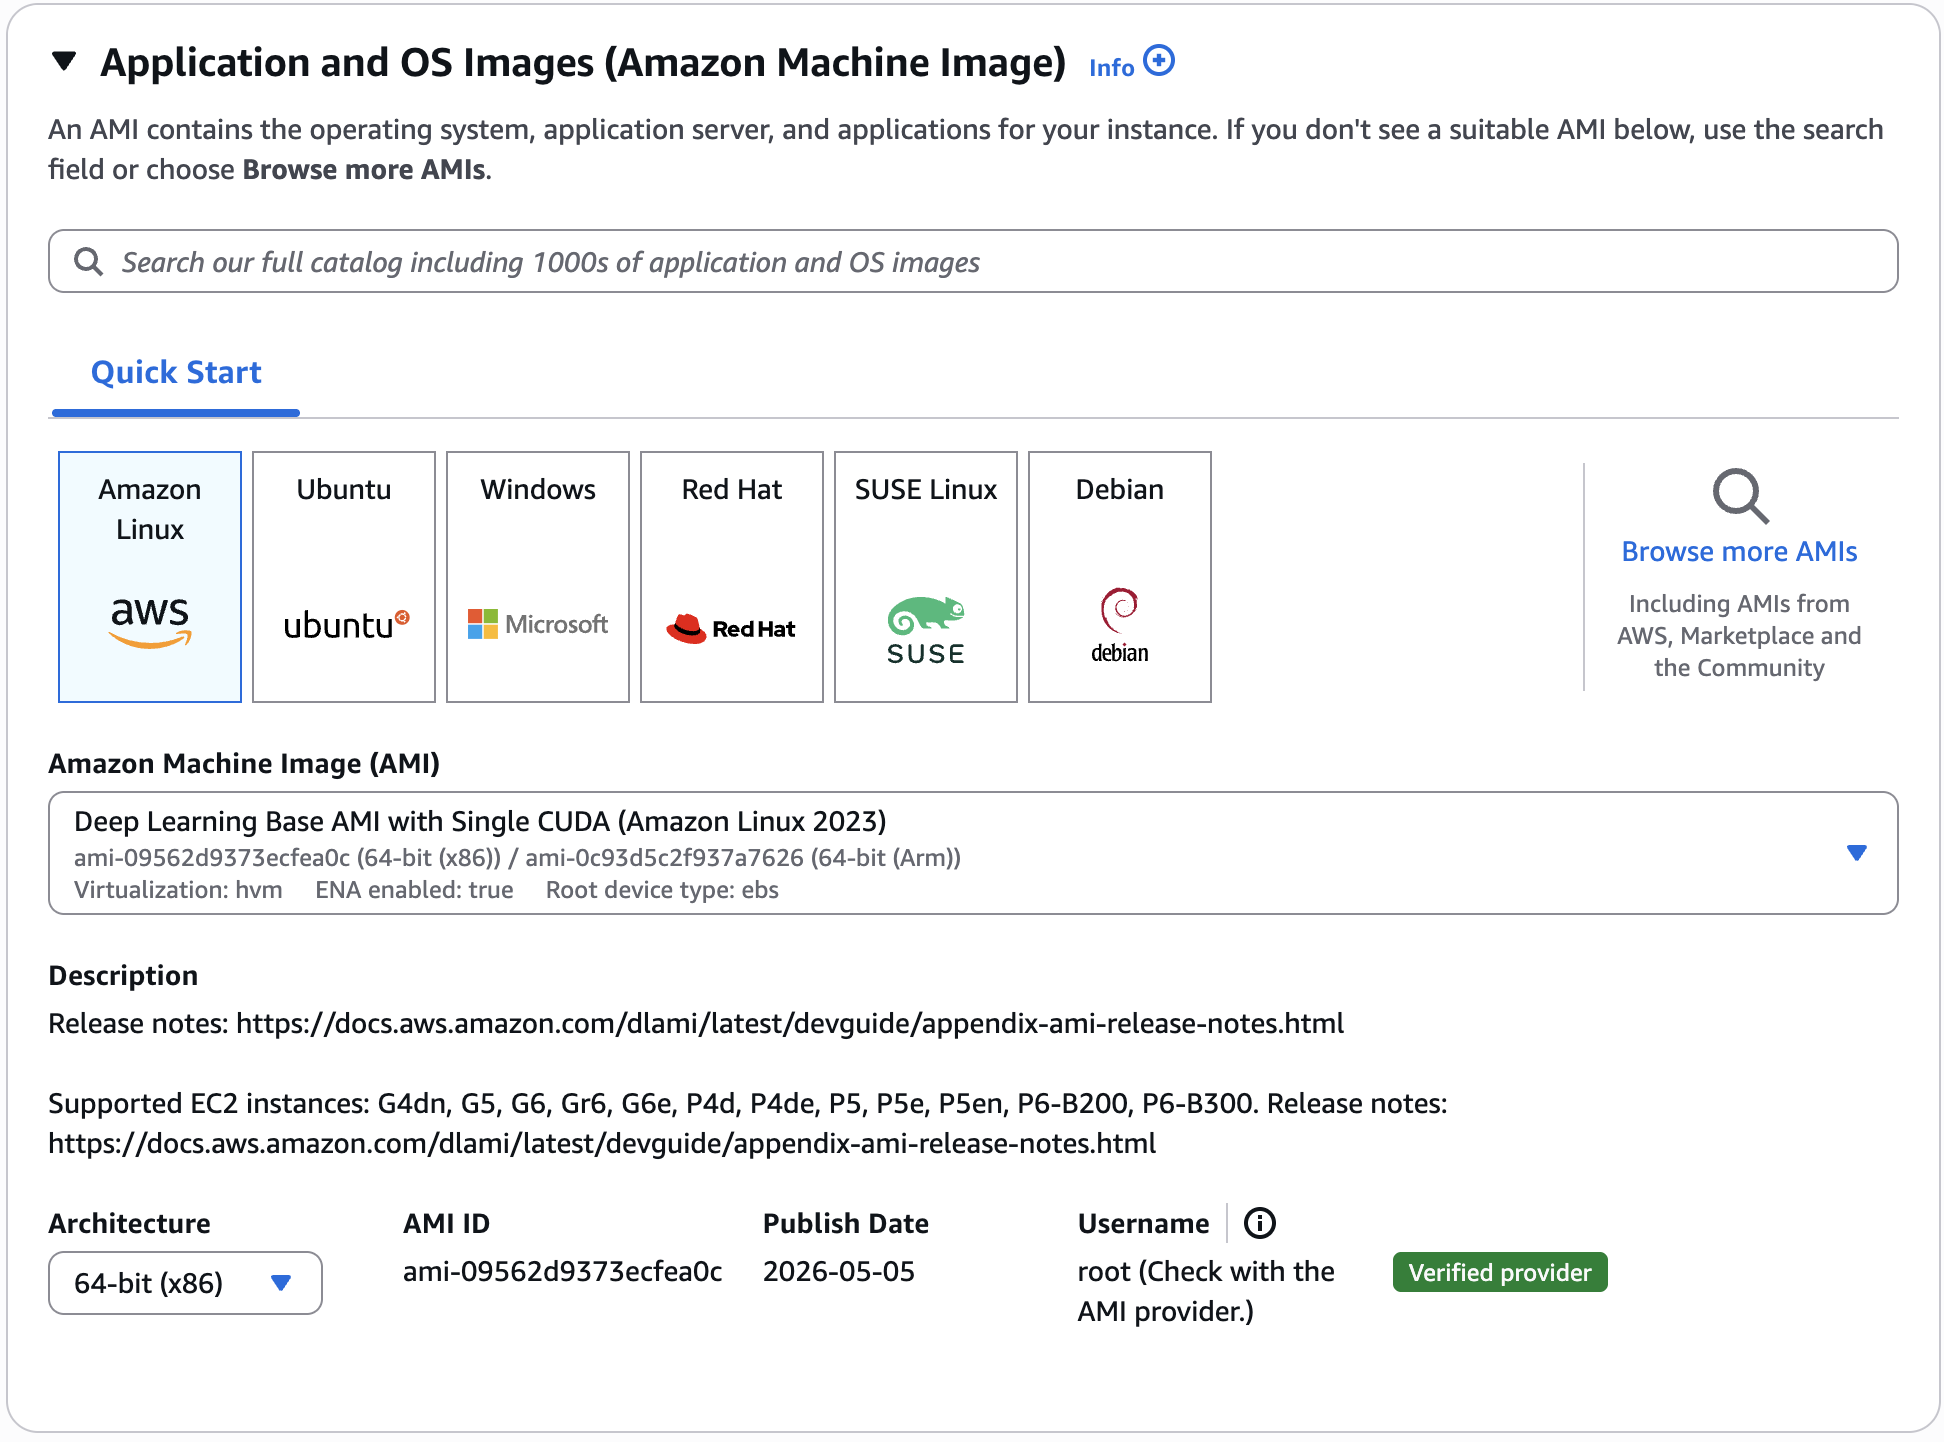
\includegraphics[width=0.8\textwidth]{images/aws_infrastructure/AMI.png}
    \caption{Selección automatizada de la AMI especializada para Deep Learning mediante Terraform.}
    \label{fig:aws_ami}
\end{figure}

\subsection{Optimización de Memoria: Batching y Aprovechamiento de VRAM}
Con el hardware desplegado, se procede a ajustar el software para aprovechar la VRAM disponible en cada fase del proyecto. Las pruebas de configuración se realizaron inicialmente sobre la NVIDIA L4 (24 GB) y se trasladaron progresivamente a la RTX PRO 6000 (96 GB) para el entrenamiento final.

\subsubsection{Estrategia de Gradient Accumulation}
Se utiliza la técnica de acumulación para simular lotes grandes sin saturar la VRAM. La Tabla \ref{tab:training_configs} resume la evolución desde el error inicial hasta la configuración óptima alcanzada durante las pruebas de estrés sobre la NVIDIA L4. La configuración conservadora (batch 4, acumulación 8) resultó estable pero lenta, mientras que la configuración optimizada (batch 16, acumulación 2) alcanzó un 97\% de utilización de la GPU manteniendo la estabilidad del entrenamiento.

\begin{table}[H]
    \centering
    \begin{tabularx}{\textwidth}{|l|c|c|c|X|}
        \hline
        \textbf{Configuración} & \textbf{Batch Físico} & \textbf{Acumulación} & \textbf{Batch Efectivo} & \textbf{Resultado} \\ \hline
        Base                   & 32                    & 1                    & 32                      & Error OOM (Falla)  \\ \hline
        Conservadora           & 4                     & 8                    & 32                      & Estable (Lento)    \\ \hline
        Optimizada             & 16                    & 2                    & 32                      & Punto óptimo (97\% Util.) \\ \hline
    \end{tabularx}
    \caption{Ajustes de memoria para maximizar el uso de la GPU NVIDIA L4 en fase de experimentación.}
    \label{tab:training_configs}
\end{table}

En el entrenamiento final sobre la NVIDIA RTX PRO 6000 Server (96 GB VRAM), la misma configuración optimizada (batch 16, acumulación 2) produjo un pico de consumo de \textbf{$\approx$90 GB}, incluyendo los pesos del modelo, activaciones del forward pass, gradientes del backward pass y estados del optimizador (Adam, que mantiene dos momentos por parámetro). Este valor, cómodo dentro de los 96 GB disponibles, confirma que la RTX PRO 6000 es el hardware mínimo recomendado para entrenar este modelo con batch efectivo 32 sin restricciones.

\subsection{Evaluación de Rendimiento vs Coste}

El proyecto ejecutó \textbf{tres entrenamientos completos}, cada uno sobre una generación de hardware distinta. La decisión de migrar entre instancias no fue arbitraria: cada salto respondió a limitaciones técnicas concretas identificadas durante el entrenamiento anterior, y se justifica por las diferencias de especificación entre las tres GPU.

\subsubsection{Progresión de Hardware y Justificación Técnica}

\begin{table}[H]
\centering
\begin{tabularx}{\textwidth}{|X|c|c|c|}
\hline
\textbf{Especificación} & \textbf{NVIDIA L4} & \textbf{NVIDIA L40S} & \textbf{RTX PRO 6000} \\ \hline
Instancia AWS & \texttt{g6.2xlarge} & \texttt{g6e.2xlarge} & \texttt{g7e.2xlarge} \\ \hline
VRAM & 22 GB & 44 GB & 96 GB \\ \hline
Tipo de memoria & GDDR6 & GDDR6 & \textbf{GDDR7} \\ \hline
Bus de memoria & 192 bits & 384 bits & 512 bits \\ \hline
Núcleos CUDA & 7.424 & 18.176 & 24.064 \\ \hline
\end{tabularx}
\caption{Comparativa de especificaciones técnicas de las tres GPU empleadas en el proyecto~\cite{techpowerup2024l4,techpowerup2024l40s,techpowerup2025rtxpro6000}.}
\label{tab:gpu_specs}
\end{table}

\begin{table}[H]
\centering
\begin{tabularx}{\textwidth}{|X|c|c|c|c|c|}
\hline
\textbf{Especificación} & \textbf{L4} & \textbf{$\Delta$ L4→L40S} & \textbf{L40S} & \textbf{$\Delta$ L40S→PRO} & \textbf{RTX PRO} \\ \hline
VRAM             & 22 GB   & +100\%  & 44 GB   & +118\% & 96 GB   \\ \hline
Bus de memoria   & 192 bit & +100\%  & 384 bit & +33\%  & 512 bit \\ \hline
Tipo de memoria  & GDDR6   & ---     & GDDR6   & ---    & \textbf{GDDR7}   \\ \hline
Núcleos CUDA     & 7.424   & +145\%  & 18.176  & +32\%  & 24.064  \\ \hline
\end{tabularx}
\caption{Mejora porcentual entre generaciones de hardware para las tres especificaciones clave.}
\label{tab:gpu_delta}
\end{table}

\begin{figure}[H]
\centering
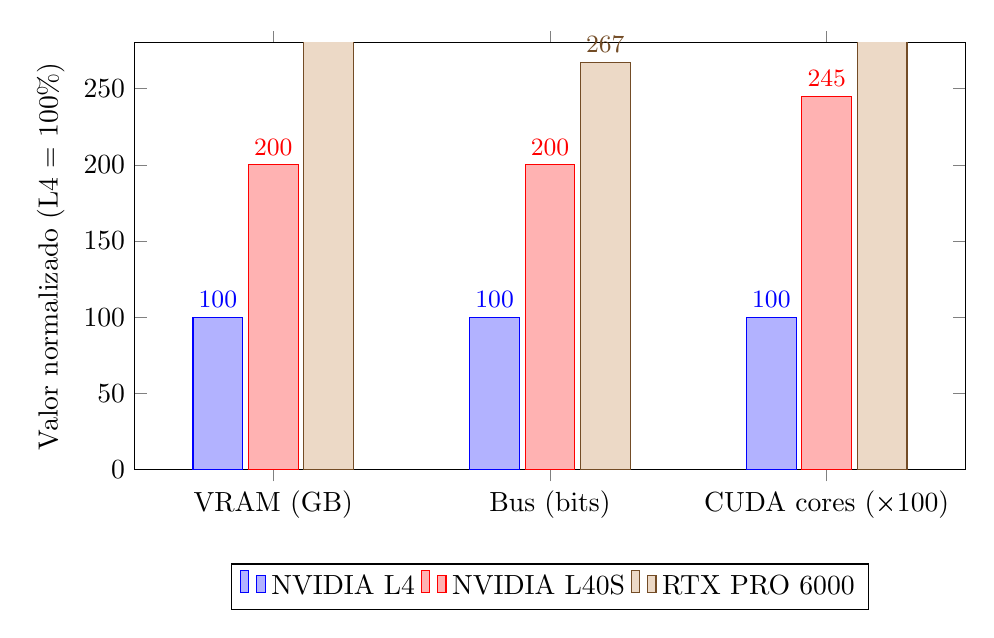
\begin{tikzpicture}
\begin{axis}[
    ybar,
    bar width=18pt,
    width=\textwidth,
    height=7cm,
    symbolic x coords={VRAM (GB), Bus (bits), CUDA cores (×100)},
    xtick=data,
    ymin=0, ymax=280,
    ylabel={Valor normalizado (L4 = 100\%)},
    legend style={at={(0.5,-0.22)}, anchor=north, legend columns=3},
    nodes near coords,
    nodes near coords align={vertical},
    every node near coord/.append style={font=\small},
    enlarge x limits=0.25,
]
\addplot coordinates {(VRAM (GB),100) (Bus (bits),100) (CUDA cores (×100),100)};
\addplot coordinates {(VRAM (GB),200) (Bus (bits),200) (CUDA cores (×100),245)};
\addplot coordinates {(VRAM (GB),436) (Bus (bits),267) (CUDA cores (×100),324)};
\legend{NVIDIA L4, NVIDIA L40S, RTX PRO 6000}
\end{axis}
\end{tikzpicture}
\caption{Rendimiento relativo de cada GPU respecto a la L4 (base = 100\%) en VRAM, ancho de bus y núcleos CUDA. La RTX PRO 6000 cuadruplica la VRAM y triplica los núcleos CUDA de la L4.}
\label{fig:gpu_comparison}
\end{figure}

\paragraph{L4 → L40S.} El bus se duplica de 192 a \textbf{384 bits} y la VRAM de 22 a \textbf{44 GB}, eliminando los errores OOM con batch sizes mayores. Los núcleos CUDA pasan de 7.424 a \textbf{18.176} (+145\%), incrementando el paralelismo de cómputo de forma sustancial.

\paragraph{L40S → RTX PRO 6000.} La VRAM vuelve a incrementarse hasta \textbf{96 GB} (+118\%), el bus alcanza \textbf{512 bits} y la memoria migra de GDDR6 a \textbf{GDDR7}, con mayor ancho de banda por pin. Los \textbf{24.064 núcleos CUDA} suponen un +32\% sobre la L40S y un +224\% acumulado sobre la L4. Esta configuración permitió alcanzar picos de $\approx$90 GB durante el entrenamiento sin restricciones.

\subsubsection{Imágenes de Precios AWS (región \texttt{eu-south-2})}

Los tres entrenamientos se facturaron en modalidad \textbf{On-Demand}, reflejando el precio real pagado por hora de cómputo.

\begin{figure}[H]
    \centering
    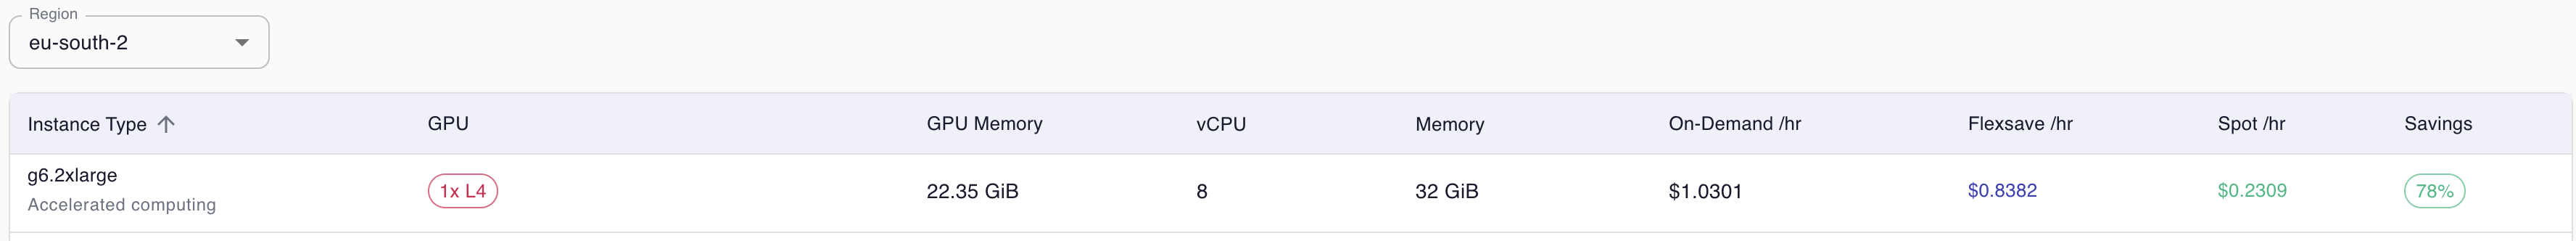
\includegraphics[width=\textwidth]{images/pricing/g6_2xlarge.png}
    \caption{Precio On-Demand de \texttt{g6.2xlarge} (NVIDIA L4): \$1,03/h. La L4 ofrece el menor coste de entrada pero su bus de 192 bits y 7.424 núcleos CUDA limitaron el throughput de entrenamiento.}
    \label{fig:pricing_g6}
\end{figure}

\begin{figure}[H]
    \centering
    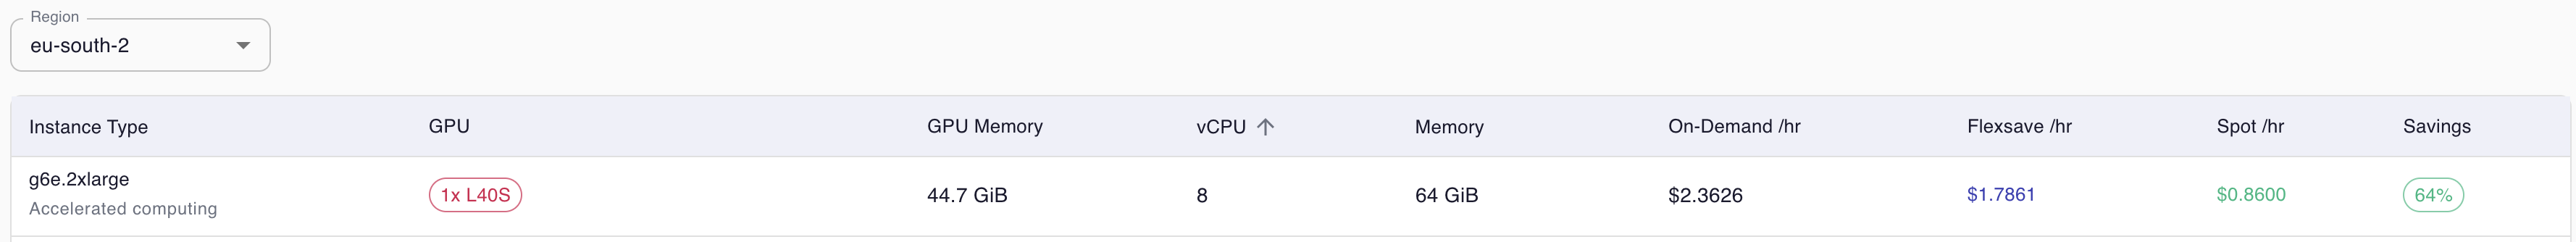
\includegraphics[width=\textwidth]{images/pricing/g6e_2xlarge.png}
    \caption{Precio On-Demand de \texttt{g6e.2xlarge} (NVIDIA L40S): \$2,36/h. Bus duplicado a 384 bits y 18.176 núcleos CUDA justifican el incremento de coste respecto a la L4.}
    \label{fig:pricing_g6e}
\end{figure}

\begin{figure}[H]
    \centering
    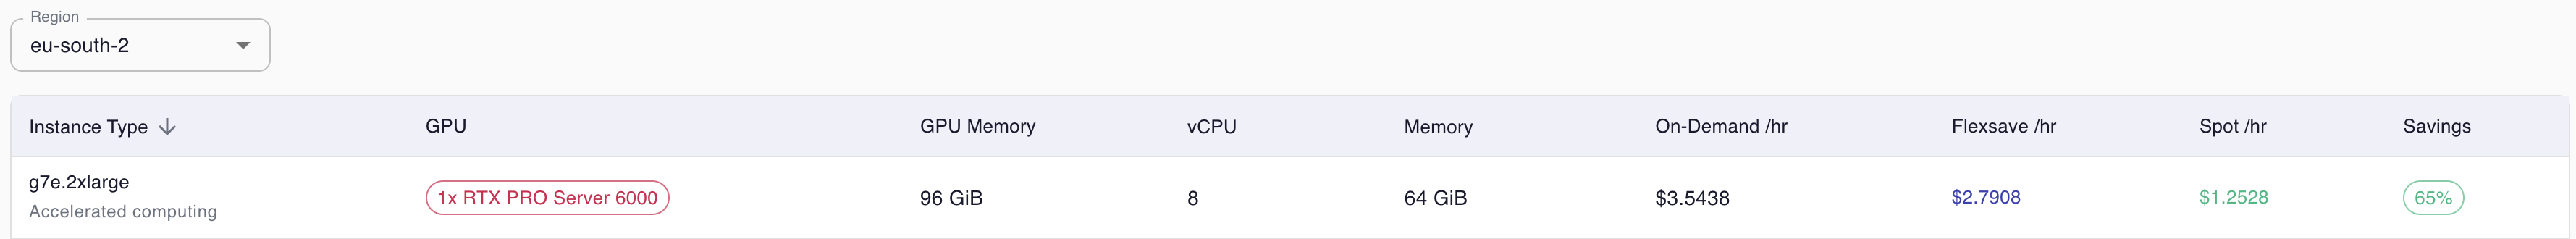
\includegraphics[width=\textwidth]{images/pricing/g7e_2xlarge.png}
    \caption{Precio On-Demand de \texttt{g7e.2xlarge} (NVIDIA RTX PRO Server 6000): \$3,54/h. Bus de 512 bits, memoria GDDR7 y 96 GB VRAM con 24.064 núcleos CUDA constituyen el hardware definitivo del proyecto.}
    \label{fig:pricing_g7e}
\end{figure}

El desglose completo de costes del proyecto, incluyendo el coste de infraestructura GPU y el coste humano, se presenta en el Capítulo~\ref{sec:costes}.

\subsection{Mejoras Iterativas de la Arquitectura durante el Entrenamiento}

A lo largo del proceso de entrenamiento se identificaron y corrigieron seis limitaciones de la arquitectura inicial mediante un ciclo de desarrollo iterativo: persistencia de estados ocultos GRU entre bloques, reposicionamiento del GRU antes de la atención (GRU → MHA → MLP), inicialización ortogonal de pesos recurrentes, gradient clipping con norma máxima 1.0, logging de contribución por componente y validación periódica contra un subconjunto no visto. El análisis detallado de cada mejora, incluyendo su justificación técnica e impacto cuantificado sobre la convergencia, se documenta en el Capítulo~\ref{sec:implementation}.

\subsection{Evolución del Hardware: De G6 a G6e y G7e}

Las optimizaciones de software descritas en las secciones anteriores exprimieron al máximo los 24 GB de VRAM de la NVIDIA L4 (\texttt{g6.2xlarge}). A medida que el batch size objetivo aumentó y los requisitos de memoria superaron ese umbral, la progresión de hardware siguió dos saltos consecutivos:

\paragraph{G6 → G6e (L4 → L40S).} Se migró a la instancia \texttt{g6e.2xlarge} equipada con la \textbf{NVIDIA L40S} (44 GB VRAM). El bus de memoria se duplica de 192 a 384 bits y la VRAM pasa de 22 a 44 GB, eliminando los errores OOM que aparecían con configuraciones de batch más agresivas. Esta instancia sirvió de paso intermedio para validar el pipeline completo con mayor holgura de memoria.

\paragraph{G6e → G7e (L40S → RTX PRO 6000).} Los requisitos del entrenamiento final de 167M parámetros con quince épocas completas superaron los 44 GB disponibles, ejecutándose la migración definitiva a la familia \textbf{G7e}, equipada con la \textbf{NVIDIA RTX PRO 6000 Server} (96 GB VRAM, bus 512 bits, memoria GDDR7). Ambas migraciones mantuvieron la misma arquitectura de despliegue basada en Terraform y Docker, sin cambios en el pipeline de entrenamiento. El entrenamiento final se ejecutó íntegramente sobre esta instancia, alcanzando picos de $\approx$90 GB durante el backward pass con batch efectivo 32.